% -*- latex -*-
%%%%%%%%%%%%%%%%%%%%%%%%%%%%%%%%%%%%%%%%%%%%%%%%%%%%%%%%%%%%%%%%
%%%%
%%%% This TeX file is part of the tutorial
%%%% `Introduction to the PETSc library'
%%%% by Victor Eijkhout, eijkhout@tacc.utexas.edu
%%%%
%%%% copyright Victor Eijkhout 2012-2022
%%%%
%%%%%%%%%%%%%%%%%%%%%%%%%%%%%%%%%%%%%%%%%%%%%%%%%%%%%%%%%%%%%%%%

\sectionframe{\texttt{Mat} Datatype: matrix}

%\subsection{Matrix basics}

\begin{numberedframe}{Matrix creation}
\small
The usual create/destroy calls:
\begin{lstlisting}
MatCreate(MPI_Comm comm,Mat *A)
MatDestroy(Mat *A)
\end{lstlisting}
Several more aspects to creation:
\begin{lstlisting}
MatSetType(A,MATSEQAIJ) /* or MATMPIAIJ or MATAIJ */
MatSetSizes(Mat A,int m,int n,int M,int N)
MatSeqAIJSetPreallocation /* more about this later*/
  (Mat B,PetscInt nz,const PetscInt nnz[])
\end{lstlisting}
Local or global size can be \lstinline{PETSC_DECIDE} (as in the vector case)
\end{numberedframe}

\begin{numberedframe}{If you already have a CRS matrix}
\begin{lstlisting}
PetscErrorCode  MatCreateSeqAIJWithArrays
  (MPI_Comm comm,PetscInt m,PetscInt n,
   PetscInt* i,PetscInt*j,PetscScalar *a,Mat *mat)
\end{lstlisting}
(also from triplets)

Do not use this unless you interface to a legacy code. And even then\ldots
\end{numberedframe}

\begin{numberedframe}{Matrix Preallocation}

  \begin{itemize}
  \item PETSc matrix creation is very flexible:
  \item No preset sparsity pattern
  \item any processor can set any element\\
    $\Rightarrow$ potential for lots of malloc calls
  \item tell PETSc the matrix' sparsity structure\\ (do construction
    loop twice: once counting, once making)
  \item Re-allocating is expensive:
\begin{lstlisting}
MatSetOption(A,MAT_NEW_NONZERO_LOCATIONS,PETSC_FALSE);
\end{lstlisting}
  (is default) Otherwise:
\begin{verbatim}
  [1]PETSC ERROR: Argument out of range
  [1]PETSC ERROR: New nonzero at (0,1) caused a malloc
\end{verbatim}
  \end{itemize}

\end{numberedframe}

\begin{numberedframe}{Sequential matrix  structure}
\begin{lstlisting}
MatSeqAIJSetPreallocation
    (Mat B,PetscInt nz,const PetscInt nnz[])
\end{lstlisting}
  \begin{itemize}
  \item \lstinline{nz} number of nonzeros per row\\ (or slight overestimate)
  \item \lstinline{nnz} array of row lengths (or overestimate)
  \item considerable savings over dynamic allocation!
  \end{itemize}
In Fortran use \lstinline{PETSC_NULL_INTEGER} if not specifying \lstinline{nnz} array
\end{numberedframe}

\begin{numberedframe}{Parallel matrix structure}
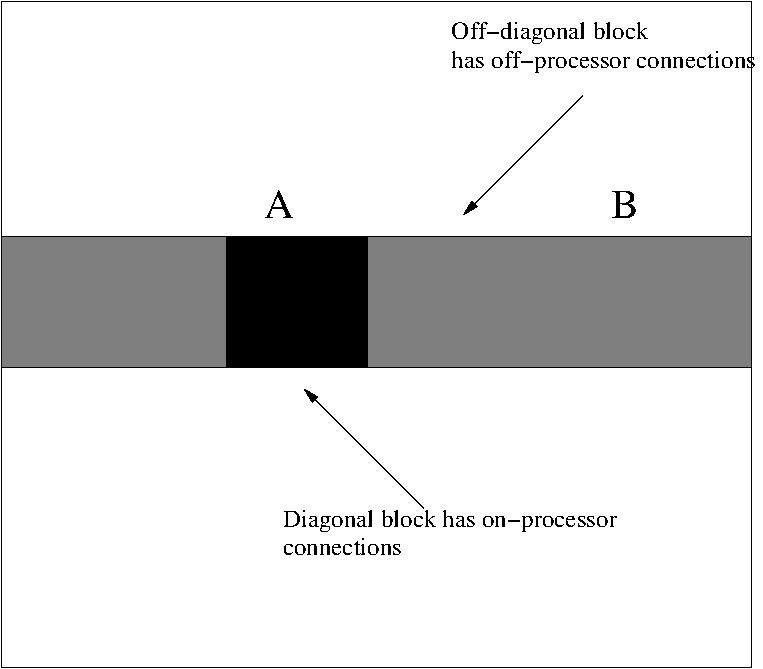
\includegraphics[scale=.5]{petscmat}
\end{numberedframe}

\begin{numberedframe}{(why does it do this?)}
  \begin{itemize}
  \item $y\leftarrow Ax_A+Bx_b$
  \item $x_B$ needs to be communicated; $Ax_A$ can be computed in the
    meantime
  \item Algorithm
    \begin{itemize}
    \item Initiate asynchronous sends/receives for $x_b$
    \item compute $Ax_A$
    \item make sure $x_b$ is in
    \item compute $Bx_B$
    \end{itemize}
  \item so by splitting matrix storage into $A,B$ part, code for the
    sequential case can be reused.
  \item This is one of the few places where PETSc's design is visible to
    the user.
  \end{itemize}
\end{numberedframe}

\begin{numberedframe}{Parallel matrix structure description}
  \begin{itemize}
  \item \lstinline{m,n} local size; \lstinline{M,N} global. Note: If the matrix is
    square, specify $m,n$ equal, even though distribution by block rows
  \item \lstinline{d_nz}: number of nonzeros per row in diagonal part
  \item \lstinline{o_nz}: number of nonzeros per row in off-diagonal part
  \item \lstinline{d_nnz}: array of numbers of nonzeros per row in diagonal part
  \item \lstinline{o_nnz}: array of numbers of nonzeros per row in off-diagonal part
  \end{itemize}
\begin{lstlisting}
MatMPIAIJSetPreallocation
  (Mat B,
   PetscInt d_nz,const PetscInt d_nnz[],
   PetscInt o_nz,const PetscInt o_nnz[])
\end{lstlisting}

In Fortran use \lstinline{PETSC_NULL_INTEGER} if not specifying arrays
\end{numberedframe}

\begin{details}
\begin{numberedframe}{Matrix creation all in one}
\begin{lstlisting}
MatCreateSeqAIJ(MPI_Comm comm,PetscInt m,PetscInt n,
  PetscInt nz,const PetscInt nnz[],Mat *A)
MatCreateMPIAIJ(MPI_Comm comm,
  PetscInt m,PetscInt n,PetscInt M,PetscInt N,
  PetscInt d_nz,const PetscInt d_nnz[],
  PetscInt o_nz,const PetscInt o_nnz[],
  Mat *A)
\end{lstlisting}
\end{numberedframe}

\end{details}

\begin{numberedframe}{Querying parallel structure}

Matrix partitioned by block rows:
\begin{lstlisting}
MatGetSize(Mat mat,PetscInt *M,PetscInt* N);
MatGetLocalSize(Mat mat,PetscInt *m,PetscInt* n);
MatGetOwnershipRange(Mat A,int *first row,int *last row);
\end{lstlisting}
 In query functions, unneeded components can be specified as
 \lstinline{PETSC_NULL}.\\
 Fortran: \lstinline{PETSC_NULL_INTEGER}
\end{numberedframe}

\begin{numberedframe}{Setting values}

Set one value:
\begin{lstlisting}
MatSetValue(Mat A,
  PetscInt i,PetscInt j,PetscScalar va,InsertMode mode)
\end{lstlisting}
where insert mode is \lstinline{INSERT_VALUES}, \lstinline{ADD_VALUES}

Set block of values:
\begin{lstlisting}
MatSetValues(Mat A,int m,const int idxm[],
    int n,const int idxn[],const PetscScalar values[],
    InsertMode mode)
\end{lstlisting}
(\lstinline{v} is row-oriented)
\end{numberedframe}

\begin{numberedframe}{Set only one element}
\begin{lstlisting}
MatSetValue(A,i,j,&v,INSERT_VALUES);
\end{lstlisting}
Special case of the general case:
\begin{lstlisting}
MatSetValues(A,1,&i,1,&j,&v,INSERT_VALUES);
\end{lstlisting}
\end{numberedframe}

\begin{numberedframe}{Assembling the matrix}
Setting elements is independent of parallelism; move elements to
proper processor:
\begin{lstlisting}
MatAssemblyBegin(Mat A,MAT_FINAL_ASSEMBLY);
MatAssemblyEnd(Mat A,MAT_FINAL_ASSEMBLY);
\end{lstlisting}

Cannot mix inserting/adding values: need to do assembly in between
with \lstinline{MAT_FLUSH_ASSEMBLY}
\end{numberedframe}

\begin{exerciseframe}[matvec]
  Pretend that you do not know how the matrix is created. Use
  \lstinline{MatGetOwnershipRange} or \lstinline{MatGetLocalSize} to create a vector
  with the same distribution, and then compute $y\leftarrow Ax$.

  (Part of the code has been disabled with \verb+#if 0+. We will get
  to that next.)
\end{exerciseframe}

\begin{details}
\begin{numberedframe}{Getting values (C)}
  \begin{itemize}
  \item Values are often not needed: many matrix operations supported
  \item Matrix elements can only be obtained locally.
  \end{itemize}
\begin{lstlisting}
PetscErrorCode  MatGetRow(Mat mat,
 PetscInt row,PetscInt *ncols,const PetscInt *cols[],
 const PetscScalar *vals[])
PetscErrorCode MatRestoreRow(/* same parameters */
\end{lstlisting}
Note: for inspection only; possibly expensive.
\end{numberedframe}

\begin{fortran}
\begin{numberedframe}{Getting values (F)}
\begin{lstlisting}
  MatGetRow(A,row,ncols,cols,vals,ierr)
  MatRestoreRow(A,row,ncols,cols,vals,ierr)
\end{lstlisting}
where \lstinline{cols(maxcols), vals(maxcols)} are long enough arrays
(allocated by the user)
\end{numberedframe}
\end{fortran}

\begin{exerciseframe}[matvec]
  Advanced exercise: create a sequential (uni-processor)
  vector. Question: how does the code achieve this?
  Give it the data of the distributed vector. Use that to compute the
  vector norm on each process separately.

  (Start by removing the \verb+#if 0+ and \verb+#endif+.)
\end{exerciseframe}

\begin{numberedframe}{Other matrix types}

\lstinline{MATBAIJ} : blocked matrices (dof per node)

(see \n{PETSC_DIR/include/petscmat.h})

Dense:
\begin{lstlisting}
MatCreateSeqDense(PETSC_COMM_SELF,int m,int n,
  PetscScalar *data,Mat *A);
MatCreateDense(MPI_Comm comm,
  PetscInt m,PetscInt n,PetscInt M,PetscInt N,
  PetscScalar *data,Mat *A)
fg\end{lstlisting}
Data argument optional:
\lstinline{PETSC_NULL} or \lstinline{PETSC_NULL_SCALAR} causes allocation
\end{numberedframe}

\begin{numberedframe}{GPU support}
  \begin{itemize}
  \item Create as GPU matrix,
  \item Otherwise transparent through overloading
  \end{itemize}
\cverbatimsnippet{pcudainit}
\indexpetscdef{VECCUDA},
\indexpetscdef{MatCreateDenseCUDA},
\indexpetscdef{MATAIJCUSPARSE}
\end{numberedframe}

\begin{numberedframe}{}
  \cverbatimsnippet{matcreatecuda}
\end{numberedframe}

\begin{comment}
  \begin{numberedframe}{}
    \cverbatimsnippet{pccudaallocsp}
  \end{numberedframe}
\end{comment}

\end{details}

\begin{numberedframe}{Matrix operations}
Main operations are matrix-vector:
\begin{lstlisting}
MatMult(Mat A,Vec in,Vec out);
MatMultAdd
MatMultTranspose
MatMultTransposeAdd
\end{lstlisting}

Simple operations on matrices:
\begin{lstlisting}
MatNorm

MatScale
MatDiagonalScale
\end{lstlisting}
\end{numberedframe}

\begin{numberedframe}{Some matrix-matrix operations}
\begin{lstlisting}
 MatMatMult(Mat,Mat,MatReuse,PetscReal,Mat*);

 MatPtAP(Mat,Mat,MatReuse,PetscReal,Mat*);

 MatMatMultTranspose(Mat,Mat,MatReuse,PetscReal,Mat*);

 MatAXPY(Mat,PetscScalar,Mat,MatStructure);
\end{lstlisting}
\end{numberedframe}

\begin{details}
\begin{numberedframe}{Matrix viewers}
\begin{lstlisting}
MatView(A,PETSC_VIEWER_STDOUT_WORLD);

row 0: (0, 1)  (2, 0.333333)  (3, 0.25)  (4, 0.2)
row 1: (0, 0.5)  (1, 0.333333)  (2, 0.25)  (3, 0.2)
....
\end{lstlisting}
(Fortran: \lstinline{PETSC_NULL_INTEGER})
  \begin{itemize}
  \item also invoked by \n{-mat_view}
  \item Sparse: only allocated positions listed
  \item other viewers: for instance \n{-mat_view_draw} (X~terminal)
  \end{itemize}

\end{numberedframe}

\end{details}

\begin{numberedframe}{General viewers}
  Any PETSc object can be `viewed'
  \begin{itemize}
  \item Terminal output: useful for vectors and matrices but also for
    solver objects.
  \item Binary output: great for vectors and matrices.
  \item Viewing can go both ways: load a matrix from file or URL into
    an object.
  \item Viewing through a socket, to Matlab or Mathematica, HDF5, VTK.
  \end{itemize}
\begin{lstlisting}
PetscViewer fd;
PetscViewerCreate( comm, &fd );
PetscViewerSetType( fd,PETSCVIEWERVTK );
MatView( A,fd );
PetscViewerDestroy(fd);
\end{lstlisting}
\end{numberedframe}

%% \begin{exerciseframe}[viewer]
%%   Fill in the blanks.
%% \end{exerciseframe}

%\subsection{Shell matrices}

\begin{numberedframe}{Shell matrices}
What if the matrix is a user-supplied operator, and not stored?

\begin{lstlisting}
MatSetType(A,MATSHELL); /* or */
MatCreateShell(MPI Comm comm,
    int m,int n,int M,int N,void *ctx,Mat *mat);

PetscErrorCode UserMult(Mat mat,Vec x,Vec y);

MatShellSetOperation(Mat mat,MatOperation MATOP_MULT,
  (void(*)(void)) PetscErrorCode (*UserMult)(Mat,Vec,Vec));
\end{lstlisting}
Inside iterative solvers, PETSc calls \lstinline{MatMult(A,x,y)}: \\
no difference between stored matrices and shell matrices
\end{numberedframe}

\begin{numberedframe}{Shell matrix context}
Shell matrices need custom data
\begin{lstlisting}
MatShellSetContext(Mat mat,void *ctx);
MatShellGetContext(Mat mat,void **ctx);
\end{lstlisting}
(This does not work in Fortran: use Common or Module
or write interface block)

User program sets context, matmult routine accesses it
\end{numberedframe}

\begin{numberedframe}{Shell matrix example}
\begin{lstlisting}
...
MatSetType(A,MATSHELL);
MatShellSetOperation(A,MATOP_MULT,(void*)&mymatmult);
MatShellSetContext(A,(void*)&mystruct);
...

PetscErrorCode mymatmult(Mat mat,Vec in,Vec out)
{
  PetscFunctionBegin;
  MatShellGetContext(mat,(void**)&mystruct);
  /* compute out from in, using mystruct */
  PetscFunctionReturn(0);
}
\end{lstlisting}
\end{numberedframe}

%\subsection{More matrix topics}

\begin{numberedframe}{Submatrices}
Extract one parallel submatrix:
\begin{lstlisting}
MatGetSubMatrix(Mat mat,
  IS isrow,IS iscol,PetscInt csize,MatReuse cll,
  Mat *newmat)
\end{lstlisting}
Extract multiple single-processor matrices:
{\small
\begin{lstlisting}
MatGetSubMatrices(Mat mat,
  PetscInt n,const IS irow[],const IS icol[],MatReuse scall,
  Mat *submat[])
\end{lstlisting}
}
Collective call, but different index sets per processor
\end{numberedframe}

\begin{numberedframe}{Load balancing}

\begin{lstlisting}
MatPartitioningCreate
    (MPI_Comm comm,MatPartitioning *part);
\end{lstlisting}
Various packages for creating better partitioning: Chaco, Parmetis

% MatCreateMPIAdj(MPI Comm comm,int mlocal,int n,const int ia[],const int ja[],
% int *weights,Mat *Adj);
% MatPartitioningCreate(MPI Comm comm,MatPartitioning *part);
% MatPartitioningSetAdjacency(MatPartitioning part,Mat Adj);
% MatPartitioningSetFromOptions(MatPartitioning part);
% MatPartitioningApply(MatPartitioning part,IS *is);
% MatPartitioningDestroy(MatPartitioning part);
% MatDestroy(Mat Adj);
% ISPartitioningToNumbering(IS is,IS *isg);


\end{numberedframe}

\endinput

\subsection{Example}

\begin{numberedframe}{Example: stencil matrices}
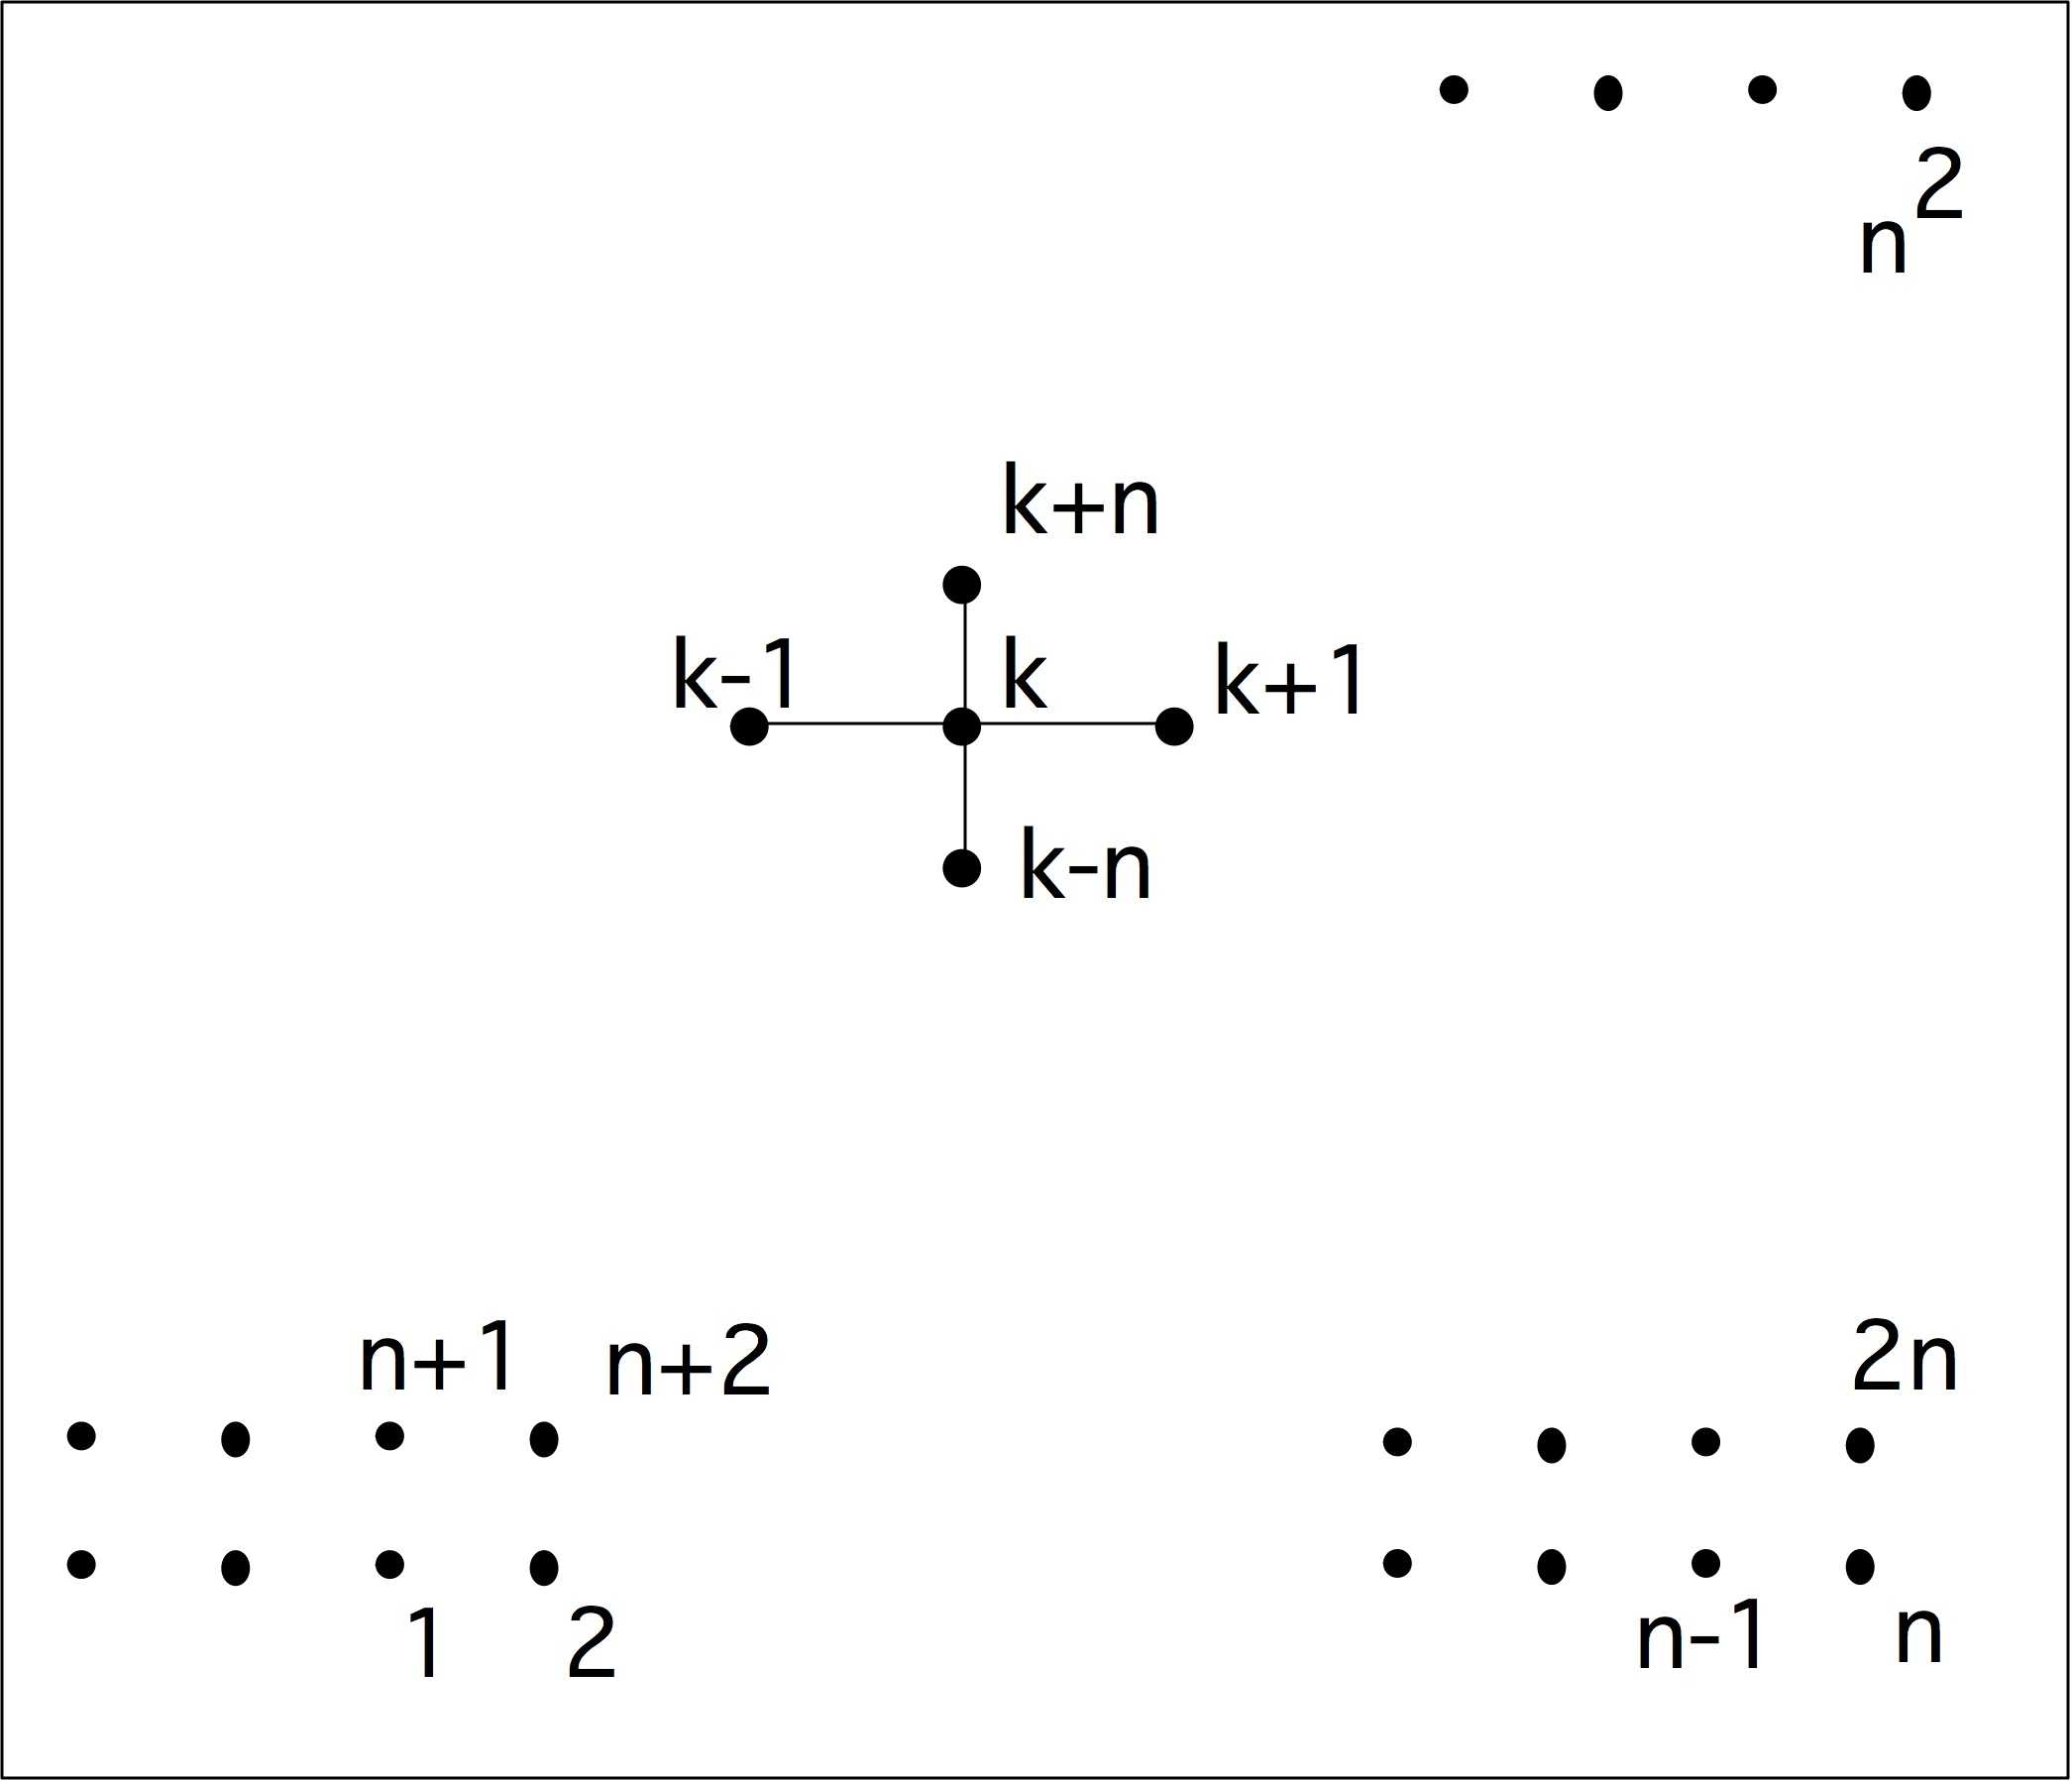
\includegraphics[scale=.6]{laplacedomain}
domain, gives matrix:
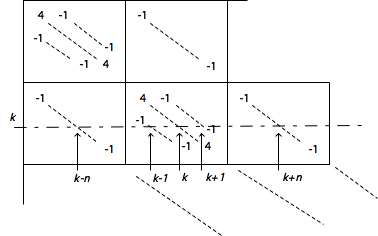
\includegraphics[scale=.6]{laplacematrix}
\end{numberedframe}

\begin{numberedframe}{Example: stencil matrices}
\small
\begin{lstlisting}
for ( i=0; i<m; i++ ) {
  for ( j=0; j<n; j++ ) {
    v = -1.0;  I = j + n*i;
    if ( i>0 ) {
        J = I - n;
        ierr = MatSetValues(mat,1,&I,1,&J,&v,INSERT_VALUES);
    }
    if ( i<m-1 ) {
        J = I + n;
        ierr = MatSetValues(mat,1,&I,1,&J,&v,INSERT_VALUES);
    }
    if ( j>0 )   { /* blah */
    if ( j<n-1 ) { /* blah */
    v = 4.0;
    ierr = MatSetValues(mat,1,&I,1,&I,&v,INSERT_VALUES);
  }
}
\end{lstlisting}
\end{numberedframe}

\begin{numberedframe}{Matrices from user data}
\footnotesize
\begin{lstlisting}
MatCreateSeqAIJWithArrays(MPI_Comm comm,
  PetscInt m,PetscInt n,
  PetscInt* i,PetscInt*j,PetscScalar *a,Mat *mat)
MatCreateMPIAIJWithArrays(MPI_Comm comm,
  PetscInt m,PetscInt n,PetscInt M,PetscInt N,
  const PetscInt i[],const PetscInt j[],const PetscScalar a[],
  Mat *mat)
MatCreateMPIAIJWithSplitArrays(MPI_Comm comm,
  PetscInt m,PetscInt n,PetscInt M,PetscInt N,
  PetscInt i[],PetscInt j[],PetscScalar a[],
  PetscInt oi[], PetscInt oj[],PetscScalar oa[],
  Mat *mat)
\end{lstlisting}
Data is copied in the 2nd case.
\end{numberedframe}

\begin{shortversion}
\begin{numberedframe}{More matrix topics}
  \begin{itemize}
  \item Viewers are also for binary dump, plotting with~X
  \item Shell matrices: matrix-free operation
  \item Submatrix extraction
  \item Matrix partitioning for load balancing
  \end{itemize}
\end{numberedframe}

\end{shortversion}
